%----------------------------------------------------------------------------------------------------------
% 	Copyright (c) 2009 R-forge 'distributions' Core Team, 
% 	
%	The following Sweave code is under the GNU Free Documentation License:
%      	Permission is granted to copy, distribute and/or modify this document
%      	under the terms of the GNU Free Documentation License, Version 1.3
%      	or any later version published by the Free Software Foundation;
%      	with no Invariant Sections, no Front-Cover Texts, and no Back-Cover Texts.
%
%      A copy of the license is included in the 'inst' directory of this package 
%      or on the web at http://www.gnu.org/licenses/licenses.html#FDL
%
%	After running Sweave, the following code could be compiled :
%	  - on windows with a Tex distribution such as miktex (http://miktex.org) 
%		and a front end Latex editor such as texniccenter (http://www.toolscenter.org)
%	  - on mac os with a Tex distribution such as TexLive and a front end Latex
%	  	editor such as Texshop (http://www.uoregon.edu/~koch/texshop/)
%	  - on linux with a Tex distribution such as teTex (http://www.tug.org/teTeX/)
%	  	and a front end Latex editor such as emacs (http://www.gnu.org/software/emacs/)
%
%----------------------------------------------------------------------------------------------------------

\chapter{The Gaussian family}
%%%%%%%%%%%%%%%%%%%%%%%%%%%%%%%%%%%%%%%%%%%%%%%%%
\section{The Gaussian (or normal) distribution}


The normal distribution comes from the study of astronomical data by the German mathematician Gauss. That's why it is widely called the Gaussian distribution. But there are some hints to think that Laplace has also used this distribution. Thus sometimes we called it the Laplace Gauss distribution, a name introduced by K. Pearson who wants to avoid a querelle about its name.


\subsection{Characterization}
\begin{wrapfigure}{r}{0.5\textwidth}
  \begin{center}
    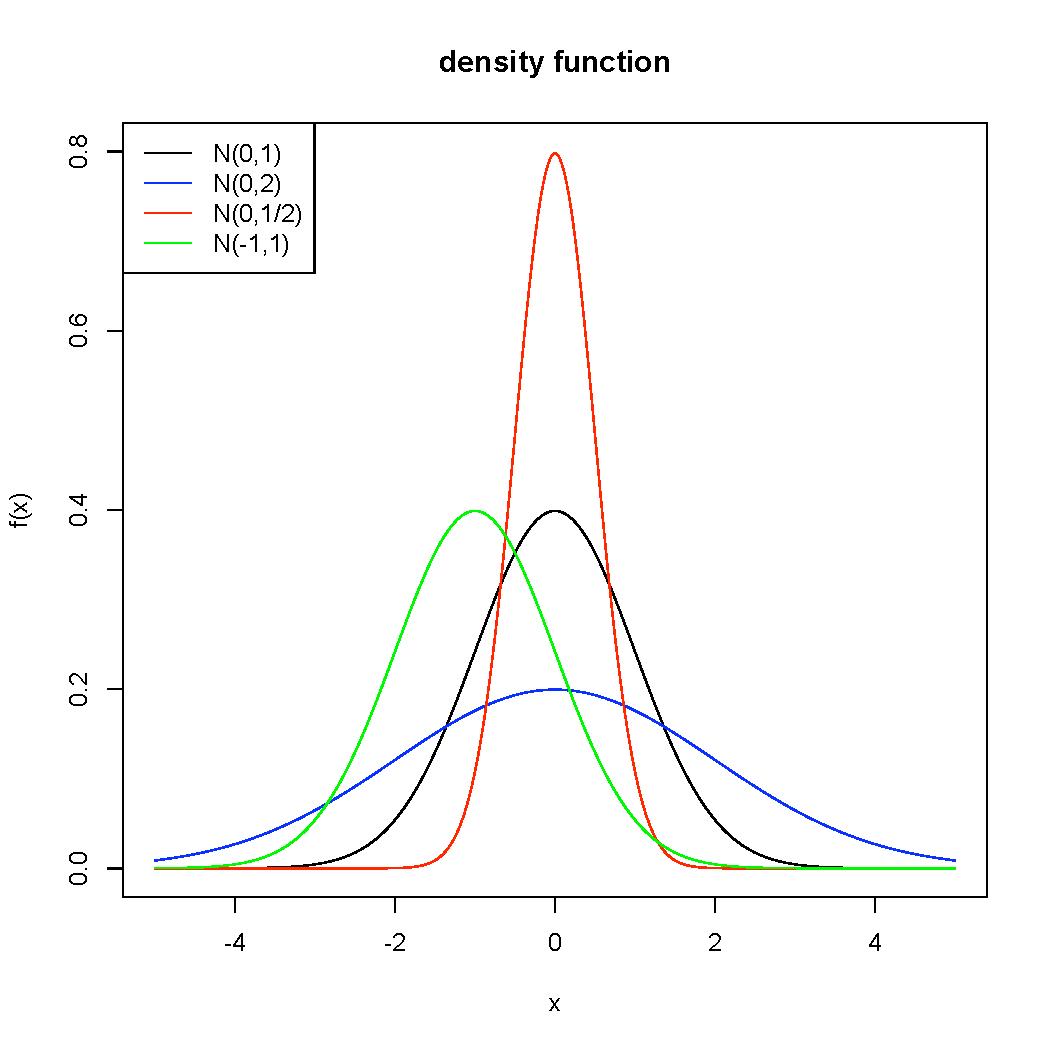
\includegraphics[width=0.48\textwidth]{img/normzoom}
  \end{center}
  \caption{The density of Gaussian distributions}
\end{wrapfigure}

The density of a normal distribution $\mathcal N(\mu, \sigma^2)$ is 
$$
f(x) =  \frac{1}{\sigma\sqrt{2\pi}} \,e^{ -\frac{(x- \mu)^2}{2\sigma^2}},
$$
where $x\in \mathbb R$ and $\mu (\in \mathbb R)$ denotes the mean of the distribution (a location parameter) and $\sigma^2 (>0)$ its variance (a scale parameter).



Its distribution function is then
$$
F(x) = \int_{-\infty}^x \frac{1}{\sigma\sqrt{2\pi}} \,e^{ -\frac{(x- \mu)^2}{2\sigma^2}} \,du,
$$
which has no explicit expressions. Many softwares have this distribution function implemented, since it is The basic distribution. Generally, we denote by $\Phi$ the distribution function a $\mathcal N(0, 1)$ normal distribution, called the standard normal distribution. $F$ can be rewritten as
$$
F(x) = \Phi\left(\frac{x-\mu}{\sigma}\right).
$$

Finally, the normal distribution can also be characterized through its moment generating function
$$
M(t) = e^{mt + \frac{\sigma^2t^2}{2}},
$$
as well as its characteristic function
$$
\phi(t) = e^{imt - \frac{\sigma^2t^2}{2}}.
$$

\subsection{Properties}
It is obvious, but let us recall that the expectation (and the median) of a normal distribution $ \mathcal N(\mu, \sigma^2)$ is $\mu$ and its variance $\sigma^2$. Furthermore if $X\sim \mathcal N(0, 1)$ we have that $E(X^n) = 0$ if $x$ is odd and $\frac{(2n)!}{2^n n!}$ if $x$ is even.



The biggest property of the normal distribution is the fact that the Gaussian belongs to the family of stable distribution (i.e. stable by linear combinations). Thus we have
\begin{itemize}
\item if $X\sim \mathcal N(\mu, \sigma^2)$ and $Y\sim \mathcal N(\nu, \rho^2)$, then $aX+bY\sim\mathcal N(a\mu+b\nu, a^2\sigma^2+b^2\rho^2+2abCov(X,Y))$, with the special case where $X,Y$ are independent cancelling the covariance term.
\item if $X\sim \mathcal N(\mu, \sigma^2)$, $a,b$ two reals, then $aX+b\sim \mathcal N(a\mu+b, a^2\sigma^2)$.
\end{itemize}

If we consider an i.i.d. sample of $n$ normal random variables $(X_i)_{1\leq i\leq n}$, then the sample mean $\overline X_n$ follows a $\mathcal N(\mu, \frac{\sigma^2}{n})$ independently from the sample variance $S^2_n$ such that $\frac{S_n^2 n}{\sigma^2}$ follows a chi-square distribution with $n-1$ degrees of freedom.

A widely used theorem using a normal distribution is the central limit theorem:\\
If $(X_i)_{1\leq i\leq n}$ are i.i.d. with mean $m$ and finite variance $s^2$, then
$\frac{\sum_{i=1}^n X_i - nm}{s\sqrt{n}} \stackrel{\mathcal L}{\longrightarrow} \mathcal N(0,1)$. If we drop the hypothesis of identical distribution, there is still an asymptotic convergence (cf. theorem of Lindeberg-Feller).


\subsection{Estimation}
The maximum likelihood estimators are 
\begin{itemize}
\item $ \overline X_n = \frac{1}{n} \sum_{i=1}^n X_i \sim \mathcal N(\mu, \frac{\sigma^2}{n})$ is the unbiased estimator with minimum variance of $\mu$,
\item $S^2_n = \frac{1}{n-1} \sum_{i=1}^n (X_i- \overline X_n)^2 \sim \chi_{n-1}^2$ is the unbiased estimator with minimum variance of $\sigma^2$\footnote{This estimator is not the maximum likelihood estimator since we unbias it.},
\item $\hat \sigma_n = \sqrt{\frac{n-1}{2}}\frac{\Gamma(\frac{n-1}{2})}{\Gamma(\frac{n}{2})} \sqrt{S_n^2}$ is the unbiased estimator with minimum variance of $\sigma$ but we generally use $\sqrt{S_n^2}$.
\end{itemize}

Confidence intervals for these estimators are also well known quantities
\begin{itemize}
\item $I(\mu) = \left[\overline X_n - \sqrt{\frac{S_n^2}{n}} t_{n-1,\alpha/2}; \overline X_n + \sqrt{\frac{S_n^2}{n}} t_{n-1,\alpha/2}\right]$,
\item $I(\sigma^2) = \left[\frac{S_n^2 n}{ z_{n-1,\alpha/2}}; \frac{S_n^2n}{ z_{n-1,1-\alpha/2}}\right]$,
\end{itemize}
where $t_{n-1,\alpha/2}$ and $z_{n-1,\alpha/2}$ are quantiles of the Student and the Chi-square distribution.

\subsection{Random generation}
The Box-Muller algorithm produces normal random variates:
\begin{itemize}
\item generate $U,V$ from a uniform $\mathcal U(0,1)$ distribution,
\item compute $X = \sqrt{-2\log U} \cos(2\pi V)$ and $Y = \sqrt{-2\log U} \sin(2\pi V)$.
\end{itemize}
In outputs, $X$ and $Y$ follow a standard normal distribution (independently).

But there appears that this algorithm under estimates the tail of the distribution (called the Neave effect, cf. \cite{patard}), most softwares use the inversion function method, consist in computing the quantile function $\Phi^{-1}$ of a uniform variate.

\subsection{Applications}
From wikipedia, here is a list of situations where approximate normality is sometimes assumed
\begin{itemize}
\item In counting problems (so the central limit theorem includes a discrete-to-continuum approximation) where reproductive random variables are involved, such as Binomial random variables, associated to yes/no questions or Poisson random variables, associated to rare events;
\item In physiological measurements of biological specimens: logarithm of measures of size of living tissue (length, height, skin area, weight) or length of inert appendages (hair, claws, nails, teeth) of biological specimens, in the direction of growth; presumably the thickness of tree bark also falls under this category or other physiological measures may be normally distributed, but there is no reason to expect that a priori;
\item Measurement errors are often assumed to be normally distributed, and any deviation from normality is considered something which should be explained;
\item Financial variables: changes in the logarithm of exchange rates, price indices, and stock market indices; these variables behave like compound interest, not like simple interest, and so are multiplicative; or  other financial variables may be normally distributed, but there is no reason to expect that a priori;
\item Light intensity: intensity of laser light is normally distributed or thermal light has a Bose-Einstein distribution on very short time scales, and a normal distribution on longer timescales due to the central limit theorem.
\end{itemize}

%%%%%%%%%%%%%%%%%%%%%%%%%%%%%%%%%%%%%%%%%%%%%%%
\section{Log normal distribution}
\subsection{Characterization}
\begin{wrapfigure}{r}{0.5\textwidth}
  \begin{center}
    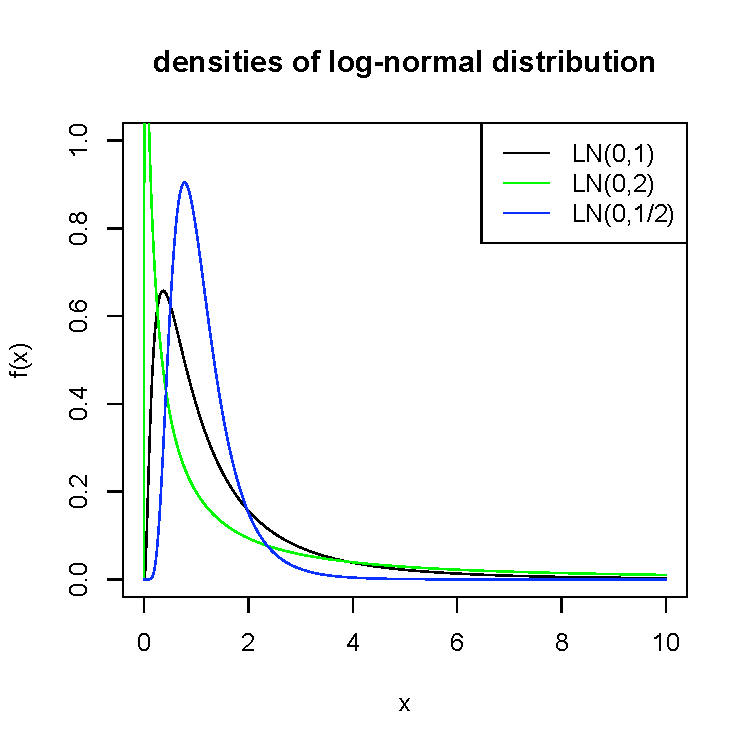
\includegraphics[width=0.48\textwidth]{img/lognormaldistrzoom}
  \end{center}
  \caption{The density of log-normal distributions}
\end{wrapfigure}

One way to characterize a random variable follows a log-normal distribution is to say that its logarithm is normally distributed. Thus the distribution function of a log-normal distribution ($\mathcal L \mathcal G(\mu,\sigma^2)$) is
$$
F(x) = \Phi\left(\frac{\log(x)-\mu}{\sigma}\right),
$$
where $\Phi$ denotes the distribution function of the standard normal distribution and $x>0$.

From this we can derive an explicit expression for the density $\mathcal L \mathcal G(\mu,\sigma^2)$
$$
f(x) =  \frac{1}{\sigma x \sqrt{2\pi}} \,e^{ -\frac{(\log(x)- \mu)^2}{2\sigma^2}},
$$
for $x>0$, $\mu\in\mathbb R$ and $\sigma^2 >0$.

A log-normal distribution does not have finite characteristic function or moment generating function.

\subsection{Properties}
The expectation and the variance of a log-normal distribution are $E(X) = e^{\mu+\frac{\sigma^2}{2}}$ and $Var(X) = (e^{\sigma^2}-1)e^{2\mu+\sigma^2}$. And raw moments are given by $E(X^n) = e^{n\mu + \frac{n^2\sigma^2}{2}}$. The median of a log-normal distribution is $e^\mu$.

From \cite{klugman}, we also have a formula for limited expected values
$$
E\left((X\wedge L)^k\right) = e^{k(\mu+\frac{k\sigma^2}{2}} \Phi(u-k\sigma) + L^k (1- \Phi(u)),
$$
where $u=\frac{\log(L)-\mu}{\sigma}$.

Since the Gaussian distribution is stable by linear combination, log-normal distribution is stable by product combination. That is to say if we consider $X$ and $Y$ two independent log-normal variables ($\mathcal L \mathcal G(\mu,\sigma^2)$ and $\mathcal L \mathcal G(\nu,\rho^2)$),
we have $XY$ follows a log-normal distribution $\mathcal L \mathcal G(\mu+\nu,\sigma^2+\rho^2)$.
Let us note that $\frac{X}{Y}$ also follows a log-normal distribution $\mathcal L \mathcal G(\mu-\nu,\sigma^2+\rho^2)$.

An equivalence of the Limit Central Theorem for the log-normal distribution is the product of i.i.d. random variables $(X_i)_{1\leq i\leq n}$ asymptotically follows a log-normal distribution with paramter $n E(\log(X))$ and $n Var(\log(X))$.

\subsection{Estimation}
Maximum likelihood estimators for $\mu$ and $\sigma^2$ are simply
\begin{itemize}
\item $\hat \mu = \frac{1}{n} \sum_{i=1}^n\log(x_i)$ is an unbiased estimator of $\mu$,
\item $\widehat{\sigma^2} = \frac{1}{n-1} \sum_{i=1}^n (\log(x_i)- \hat \mu)^2$ is an unbiased estimator of $\sigma^2$\footnote{As for the $\sigma^2$ estimator of normal distribution, this estimator is not the maximum likelihood estimator since we unbias it.}.
\end{itemize}
One amazing fact about parameter estimations of log-normal distribution is that those estimators are very stable. 

\subsection{Random generation}
Once we have generated a normal variate, it is easy to generate a log-normal variate just by taking the exponential of normal variates.

\subsection{Applications}
There are many applications of the log-normal distribution. \cite{logappli} focuses on application of the log-normal distribution. For instance, in finance the Black \& Scholes assumes that assets are log-normally distributed (cf. \cite{blackscholes73} and the extraordinary number of articles citing this article).
\cite{biolognorm} deals with environmental applications of the log-normal distribution.



%%%%%%%%%%%%%%%%%%%%%%%%%%%%%%%%%%%%%%%%%%%%%%%
\newpage\section{Shifted log normal distribution}
\subsection{Characterization}
\begin{wrapfigure}{r}{0.5\textwidth}
  \vspace{-20pt}
  \begin{center}
    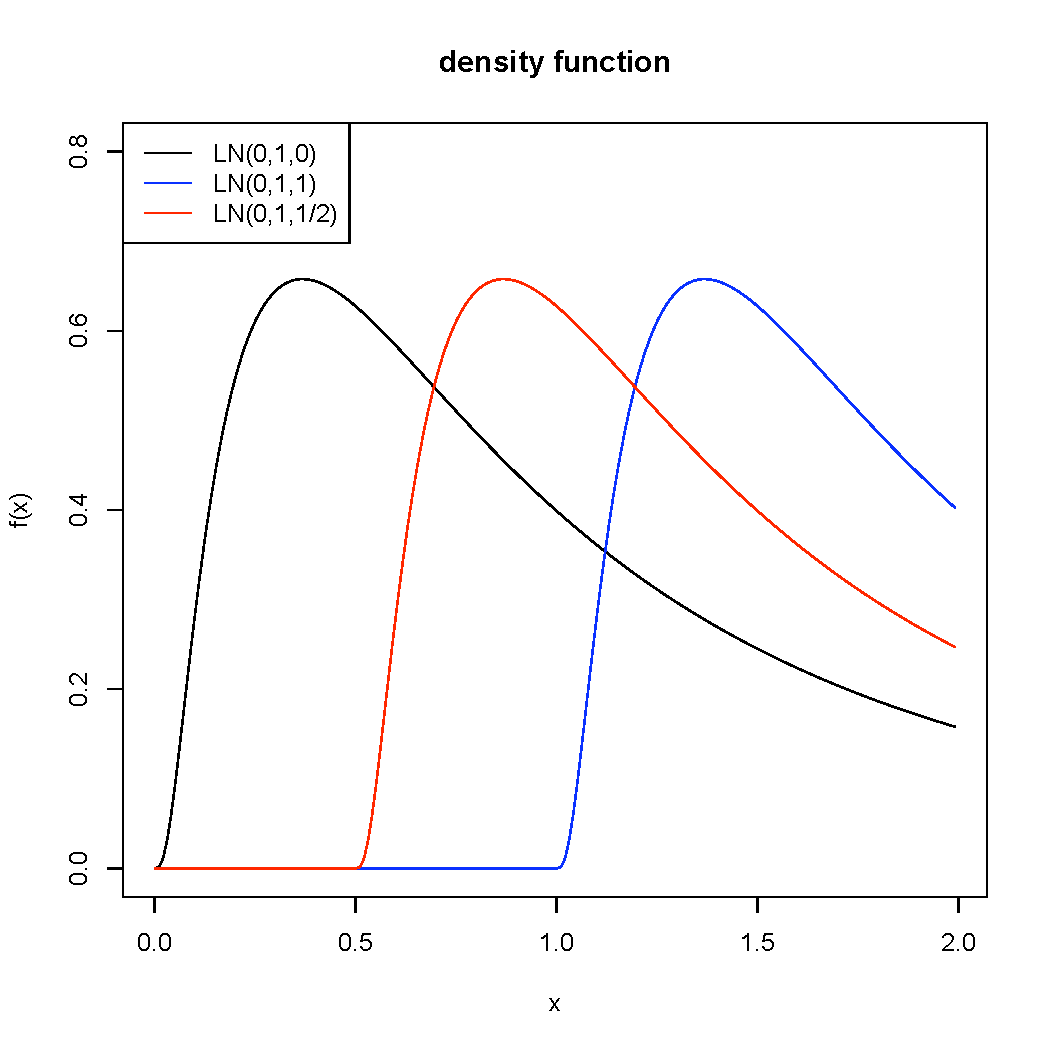
\includegraphics[width=0.48\textwidth]{img/shiftlognormzoom}
  \end{center}
  \vspace{-20pt}
  \caption{The density of shifted log-normal distributions}
  \vspace{-20pt}
\end{wrapfigure}
An extension to the log-normal distribution is the translated log-normal distribution. It is
the distribution of $X+\nu$ where $X$ follows a log-normal distribution.
It is characterized by the following distribution function
$$
F(x) = \Phi\left(\frac{\log(x-\nu)-\mu}{\sigma}\right),
$$
where $\Phi$ denotes the distribution function of the standard normal distribution and $x>0$.
Then we have this expression for the density $\mathcal T\mathcal L \mathcal G(\nu,\mu,\sigma^2)$
$$
f(x) =  \frac{1}{\sigma (x-\nu) \sqrt{2\pi}} \,e^{ -\frac{(\log(x-\nu)- \mu)^2}{2\sigma^2}},
$$
for $x>0$, $\mu,\nu\in\mathbb R$ and $\sigma^2 >0$.

As for the log-normal distribution, there is no moment generating function nor characteristic function.

\subsection{Properties}
The expectation and the variance of a log-normal distribution are $E(X) =\nu+ e^{\mu+\frac{\sigma^2}{2}}$ and $Var(X) = (e^{\sigma^2}-1)e^{2\mu+\sigma^2}$. And raw moments are given by $E(X^n) = e^{n\mu + \frac{n^2\sigma^2}{2}}$. 

\subsection{Estimation}
An intuitive approach is to estimate $\nu$ with $X_{1:n}$, then estimate parameters on shifted samples $(X_i-\nu)_i$.

\subsection{Random generation}
Once we have generated a normal variate, it is easy to generate a log-normal variate just by taking the exponential of normal variates and adding the shifted parameter $\nu$.

\subsection{Applications}
An application of the shifted log-normal distribution to finance can be found in \cite{haahtela} or
\cite{brigo}.

%%%%%%%%%%%%%%%%%%%%%%%%%%%%%%%%%%%%%%%%%%%%%%
\section{Inverse Gaussian distribution}
\subsection{Characterization}

\begin{wrapfigure}{r}{0.5\textwidth}
  \vspace{-30pt}
  \begin{center}
    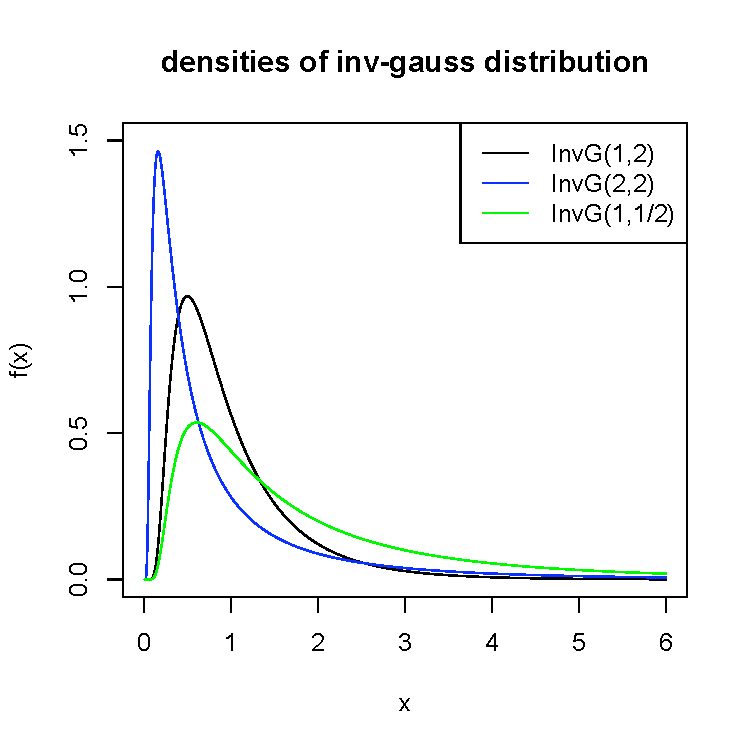
\includegraphics[width=0.48\textwidth]{img/invgaussdistrzoom}
  \end{center}
  \vspace{-20pt}
  \caption{The density of inverse Gaussian distributions}
  \vspace{-20pt}
\end{wrapfigure}

The density of an inverse Gaussian distribution $\mathcal I \mathcal G(\nu, \lambda)$ is given by
$$
f(x)=\sqrt{\frac{\lambda}{2\pi x^3}}\exp\left[-\lambda\frac{(x-\nu)^2}{2\nu^2 x}\right],
$$
while its distribution function is
$$
F(x)=\Phi\left[\sqrt{\frac{\lambda}{x}}\left(\frac{x}{\nu}-1\right)\right]+e^{2\lambda/\nu}\Phi\left[\sqrt{\frac{\lambda}{x}}\left(\frac{x}{\nu}+1\right)\right],
$$
for $x>0$, $\nu\in\mathbb R$, $\lambda>0$ and $\Phi$ denotes the usual standard normal distribution.

Its characteristic function is 
$$
\phi(t) = e^{\left(\frac{\lambda}{\nu}\right)\left[1-\sqrt{1-\frac{2\nu^2\mathrm{i}t}{\lambda}}\right]}.
$$

The moment generating function is expressed as
$$
M(t) = e^{\left(\frac{\lambda}{\nu}\right)\left[1-\sqrt{1-\frac{2\nu^2t}{\lambda}}\right]}.
$$

\subsection{Properties}
The expectation of an inverse Gaussian distribution $\mathcal I \mathcal G(\nu, \lambda)$ is
$\nu$ and its variance $\frac{\nu^3}{\lambda}$.

Moments for the inverse Gaussian distribution are given 
$E(X^n) = \nu^n \sum_{i=0}^{n-1}\frac{\Gamma(n+i)}{\Gamma(i+1)\Gamma(n-i)} (\frac{2\lambda}{\nu})^i$ for $n$ integer.

From \cite{yu}, we have the following properties
\begin{itemize}
\item if $X$ is inverse Gaussian distributed $\mcal I \mcal G(\nu, \lambda)$, then $aX$ follows an inverse Gaussian distribution $\mcal I \mcal G(a\nu, a\lambda)$ for $a>0$
\item if $(X_i)_i$ are i.i.d. inverse Gaussian variables, then the sum $\sum_{i=1}^n X_i$ still follows an inverse Gaussian distribution $\mcal I \mcal G(n\nu, n^2\lambda)$
\end{itemize}


\subsection{Estimation}
Maximum likelihood estimators of $\nu$ and $\lambda$ are
$$
\hat{\mu}= \bar X_n
\txtm{and} 
\hat{\lambda}= n \left( \sum_{i=1}^n \left( \frac1{X_i}-\frac1{\hat{\mu}} \right) \right)^{-1}.
$$
From previous properties, $\hat \mu$ follows an inverse gaussian distribution $\mcal I\mcal G(\mu,n\lambda)$ and $\frac{n\lambda}{\hat \lambda}$ follows a chi-squared distribution $\chi_{n-1}^2$.


\subsection{Random generation}
NEED 	

Mitchael,J.R., Schucany, W.R. and Haas, R.W. (1976). Generating
	random roots from variates using transformations with multiple roots.
	American Statistician. 30-2. 88-91.

\subsection{Applications}
NEED REFERENCE

%%%%%%%%%%%%%%%%%%%%%%%%%%%%%%%%%%%%%%%%%%%%%%%%%
\section{The generalized inverse Gaussian distribution} \label{sec:gig}
This section is taken from \cite{ghyp}.

\subsection{Characterization}
\begin{wrapfigure}{r}{0.5\textwidth}
  \vspace{-60pt}
  \begin{center}
    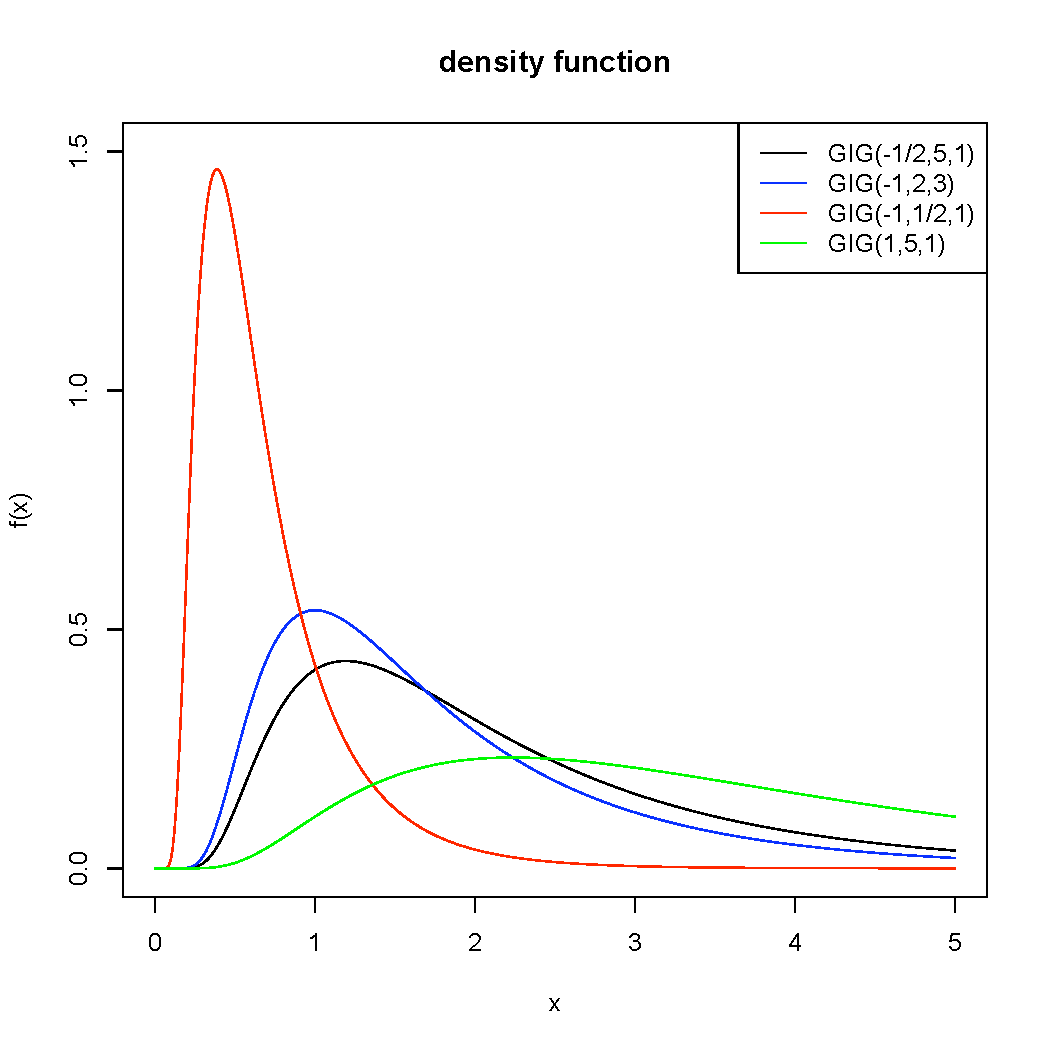
\includegraphics[width=0.48\textwidth]{img/gigzoom}
  \end{center}
  \vspace{-20pt}
  \caption{The density of generalized inverse Gaussian distributions}
  \vspace{-20pt}
\end{wrapfigure}
A generalization of the inverse Gaussian distribution exists but there is no
closed form for its distribution function and its density used Bessel functions.
The latter is as follows
$$\label{eq:densgig}
 f(x) = \left(\frac{\psi}{\chi}\right)^{\frac{\lambda}{2}}
  \frac{x^{\lambda-1}}{2K_\lambda(\sqrt{\chi\psi})} \,
  \exp\left\{-\frac{1}{2}\left(\frac{\chi}{x}+\psi x
    \right)\right\},
$$
where $x>0$ and $K_\lambda$ denotes the modified Bessel function. Parameters must satisfy
\begin{itemize}
\item $\chi > 0, \psi \geq 0$, when $\lambda < 0 $,
\item $\chi > 0, \psi > 0$, when $\lambda = 0$,
\item $\chi \geq 0, \psi > 0$, when $\lambda > 0 $.
\end{itemize} 
The generalized inverse Gaussian is noted as $\mathcal G \mathcal I \mathcal G(\lambda,\psi,\chi)$.

Closed form for distribution function??

Plot

The moment generating function is given by
\begin{equation}
  M(t) = \left(\frac{\psi}{\psi - 2 t}\right)^{\lambda / 2}
  \frac{K_\lambda(\sqrt{\chi (\psi - 2 t)})}{K_\lambda(\sqrt{\chi \psi})}.
\end{equation}


\subsection{Properties}
The expectation is given by 
$$
\sqrt{\frac{\chi}{\psi}}
  \frac{K_{\lambda+1}(\sqrt{\chi\psi})}{K_{\lambda}(\sqrt{\chi\psi})},
$$ and more generally the $n$-th moment is as follows
$$
  E(X^n) = \left(\frac{\chi}{\psi}\right)^\frac{n}{2}
  \frac{K_{\lambda+n}(\sqrt{\chi\psi})}{K_\lambda(\sqrt{\chi\psi})}.
$$
Thus we have the following variance
$$
Var(X) = \frac{\chi}{\psi}
  \frac{K_{\lambda+2}(\sqrt{\chi\psi})}{K_\lambda(\sqrt{\chi\psi})} - \frac{\chi}{\psi}
  \left(\frac{K_{\lambda+1}(\sqrt{\chi\psi})}{K_\lambda(\sqrt{\chi\psi})}\right)^2.
$$


Furthermore,
\begin{equation}\label{eq:eloggig}
  E(\log X) =  \frac{\partial d E(X^\alpha)}{\partial d \alpha}\biggr|_{\alpha=0}.
\end{equation}
Note that numerical calculations of $E(\log X)$ may be performed
with the integral representation as well.



\subsection{Estimation}
NEED REFERENCE

\subsection{Random generation}
NEED REFERENCE


